\subsubsection{Généralités}

OpenVPN est un outil Open-Source permettant de créer des tunnels sécurisés utilisant un chiffrement SSL/TLS. OpenVPN propose un client à la fois facile à installer et à configurer, en plus d'être disponible sur à peut prêt toutes les plates-formes (Linux, Windows, BSD, Mac OS, Solaris). Le principe de configuration reste le même quelque soit la plate-forme utilisée.

% 
% \subsubsection{Les deux types de VPN}
% OpenVPN propose deux types de VPN : les VPN bridgés et les VPN routés. Dans le cas du mode bridgé le réseau virtuel créé devient une réelle extension du réseau local. L'avantage de ce mode est la facilité d'intégration de la solution VPN au sein de l'infrastructure déjà en place. Ce mode est d'ailleurs la seule option si pour une raison ou pour une autre des paquets broadcasts doivent traverser le VPN. Le principal inconvénient de ce mode apparait lors du passage à l'échelle : comme c'est le réseau local qui doit absorber les clients du VPN, il faut suffisament de ressources disponibles (adresses IP, etc.).
% 
% TODO : c'est pas tout à fait vrai
% 
% Le mode routé est le mode le plus utilisé. Bien que sa mise en place soit plus complexe, ce mode permet de faire du réseau virtuel un réseau à part du réseau local. On est ainsi capable de mettre en place une politique d'accès différente pour les utilisateurs connectés depuis l'extérieur, ce qui renforce encore la sécurité de l'infrastructure. Le second grand avantage des VPN routés est que le passage a l'échelle s'effectue ne pose aucun problème étant donné que l'on n'impacte pas l'utilisation du réseau local.
% 
% ~
% 
% La figure \ref{tableau_types_vpn} résume les avantages et inconvénient de chacun des deux types de VPN :
% \begin{figure}[H]
% 	\begin{center}
% 		\begin{tabular}{c|c}
% 			VPN bridgé & VPN routé \\
% 			\hline
% 			extension du réseau local & réseau à part \\
% 			mauvais passage à l'échelle & passage à l'échelle \\
% 			laisse passer les broadcasts & broadcasts impossibles \\
% 		\end{tabular}
% 	\end{center}
% 	\caption{Avantages et inconvénients des deux types de VPN}
% 	\label{tableau_types_vpn}
% \end{figure}
% 
% Nous avons choisi de mettre en place une configuration de VPN routé, car mieux adaptée à l'utilisation que l'ISIMA pourrait en faire.

\subsubsection{Mise en place du serveur}

La mise en place de l'infrastructure s'effectue en plusieures étapes. Tout d'abord nous installerons et configurerons OpenVPN sur le serveur, ensuite nous générerons les clefs et certificats de sécurité nécessaires, et enfin nous mettrons en place les outils nécessaires pour authentifier les utilisateurs via l'annuaire NIS de l'ISIMA.

Les interfaces de la machine sont configurées comme indiqué figure \ref{schema-physique-maquette} page \ref{schema-physique-maquette}, et résumé dans le tableau figure \ref{linux_interfaces} :

\begin{figure}[H]
	\begin{center}
		\begin{tabular}{c|c|l}
			Interface & Adresse IP & Commentaire \\
			\hline
			eth0 & 192.168.0.10 & Réseau interne étudiants \\
			eth1 & 192.168.102.121 & Réseau externe \\
			eth2 & 10.0.0.10 & Réseau interne profs \\
		\end{tabular}
	\end{center}
	\caption{Configuration des interfaces de la machine Linux}
	\label{linux_interfaces}
\end{figure}


\paragraph{Installation et configuration d'OpenVPN}

\subparagraph{Résolution des dépendances}
~

La machine fonctionne sous \texttt{Linux CentOS 5.1}. OpenVPN n'étant pas disponible directement dans les paquets de cette distribution (vieille de deux ans à l'écriture de ces lignes), nous allons construire notre propre rpm. Les paquets requis pour mener à bien cette étape sont à installer grâce à la commande suivante :

\verb|[root@centosvpn ~]# yum install openssl-devel pam-devel rpm-build gcc-c++|

~

La version d'OpenVPN utilisée pour le projet est la 2.0.9 disponible sur \verb|http://openvpn.net/|. Celle-ci dépend des paquets \verb|lzo-devel-1.08-fr2.i386| et \verb|lzo-1.08-fr2.i386|, disponibles par exemple sur \verb|http://rpmfind.net/|.

\verb|[root@centosvpn ~]# wget ftp://rpmfind.net/linux/freshrpms/redhat/9/lzo/lzo-deve|

\verb|l-1.08-fr2.i386.rpm|

\verb|[root@centosvpn ~]# wget ftp://rpmfind.net/linux/freshrpms/redhat/9/lzo/lzo-1.08|

\verb|-fr2.i386.rpm|

\verb|[root@centosvpn ~]# rpm -ivh lzo-1.08-fr2.i386 lzo-devel-1.08-fr2.i386.rpm|

\subparagraph{Compiler OpenVPN}
~

Lors de la configuration de notre maquette la version courante d'OpenVPN était la 2.0.9; adaptez les numéros de version avec celui de la dernière release stable d'OpenVPN. Les commandes suivantes permettent à la fois de la récupérer, de la compiler, et de l'installer :

\verb|[root@centosvpn ~]# wget http://openvpn.net/release/openvpn-2.0.9.tar.gz|

\verb|[root@centosvpn ~]# rpmbuild -tb openvpn-2.0.9.tar.gz|

\verb|[root@centosvpn ~]# rpm -ivh /usr/src/redhat/RPMS/i386/openvpn-2.0.9-1.i386.rpm|

\subparagraph{Configuration de base}
~

Une instance d'OpenVPN ne peut gérer qu'un seul pool d'adresses à la fois, et donc un seul type de clients pour le VPN. La solution pour gérer à la fois les professeurs et les étudiants grâce à une même machine est donc de lancer deux instances du serveur en écoute sur un port différent. Nous allons donc utiliser deux fichiers de configuration distincts dont la figure \ref{configuration_base_openvpn} présente les paramètres qui leurs sont communs : Interface d'écoute, protocole de transport, etc.

Pour toute la suite nous considérerons que ces fichiers se trouvent dans le dossier \texttt{/etc/openvpn/} et portent les noms \texttt{server-prof.conf} et \texttt{server-student.conf} :

\begin{figure}[H]
	\begin{center}
		\begin{minipage}{0.90\textwidth}
			\begin{lstlisting}[frame=trBL]
local 192.168.102.121
proto udp
dev tap
client-to-client
duplicate-cn
keepalive 10 120
comp-lzo
user nobody
group nobody
persist-key
persist-tun
status openvpn-status.log
verb 3
			\end{lstlisting}
		\end{minipage}
	\end{center}
	\caption{Configuration de base d'OpenVPN}
	\label{configuration_base_openvpn}
\end{figure}

~

Pour configurer correctement deux instances qui puissent cohabiter, celles-ci doivent se mettre en écoute sur un port différent. Nous avons choisi le port 1194 (port par défaut d'OpenVPN) pour le serveur profs, ainsi que le port 1195 pour le serveur étudiant. Les figures \ref{configuration_base_prof} et \ref{configuration_base_student} détaillent également la configuration des pools d'adresses à affecter aux clients, ainsi que les informations de routage à leur transmettre :

\begin{figure}[H]
	\begin{lstlisting}[frame=trBL]
port 1194
server 10.0.1.0 255.255.255.0
ifconfig-pool-persist ipp-profs.txt
push ``route 10.0.0.0 255.255.255.0''
	\end{lstlisting}
	\caption{Configuration spécifique aux profs}
	\label{configuration_base_prof}
\end{figure}
\begin{figure}[H]
	\begin{lstlisting}[frame=trBL]
port 1195
server 192.168.1.0 255.255.255.0
ifconfig-pool-persist ipp-profs.txt
push ``route 192.168.0.0 255.255.255.0''
	\end{lstlisting}
	\caption{Configuration spécifique aux étudiants}
	\label{configuration_base_student}
\end{figure}


\paragraph{Génération des clefs et certificats de sécurité}
~

Dans cette section nous allons voir comment générer les clefs et certificats qui serviront à sécuriser les authentifications auprès du serveur OpenVPN. Pour cela nous allons utiliser une suite de scripts shell nommée \verb|easy-rsa|, une sorte de frontend pour OpenSSL. Cette suite \verb|easy-rsa| fournie avec OpenVPN permet de grandement simplifier le travail de génération et de gestion des clefs et certificats.

~

Commençons par récupérer les outils. Si OpenVPN a été compilé suivant les étapes ci-dessus, ceux-ci se trouve dans le répertoire \verb|/usr/share/openvpn/easy-rsa|. Il faut copier ce répertoire dans un lieu sûr puis ouvrir un shell à cet endroit. L'étape suivante consiste à éditer le fichier \verb|vars| pour configurer les paramètres globaux des scripts, comme indiqué figure \ref{easy-rsa-globals} :

\begin{figure}[H]
	\begin{center}
		\begin{minipage}{0.90\textwidth}
			\begin{lstlisting}[frame=trBL]
export KEY_COUNTRY=FR
export KEY_PROVINCE=FR
export KEY_CITY=``Clermont-Ferrand''
export KEY_ORG=``ISIMA''
export KEY_EMAIL=``nobody@nowhere.com''
			\end{lstlisting}
		\end{minipage}
	\end{center}
	\caption{Paramètres globaux des certificats}
	\label{easy-rsa-globals}
\end{figure}

L'environnement du shell doit ensuite être initialisé en important le contenu du fichier vars :

\verb|[root@centosvpn easy-rsa]# . ./vars|

Comme c'est notre premier lancement on s'assure que tout est propre :

\verb|[root@centosvpn easy-rsa]# ./clean-all|

~

Nous créons ensuite nos clef et certificat de CA (Certificate Authority) afin de pouvoir signer les certificats de nos clients. Seule l'entrée ``COMMON NAME'' n'est pas tirée du fichier \verb|vars|, la valeur \verb|ISIMA CA| fera très bien l'affaire :

\verb|[root@centosvpn easy-rsa]# ./build-ca|

~

Nous allons maintenant générer les clefs et certificats pour le serveur et les deux types de clients. L'entrée ``COMMON NAME'' devra être précisée de façon à prendre respectivement les valeurs ``ISIMA SERVER'', ``ISIMA PROF'' et ``ISIMA STUDENT''. De plus il faut signer chaque certificat avec notre CA et commiter le résultat dans la base OpenSSL du serveur :

\verb|[root@centosvpn easy-rsa]# ./build-key-server server|

\verb|[root@centosvpn easy-rsa]# ./build-key prof|

\verb|[root@centosvpn easy-rsa]# ./build-key student|

~

Ensuite nous initialisons un générateur de grand nombres premiers pour le procédé d'échange de clefs via la méthode Diffie Hellman :

\verb|[root@centosvpn easy-rsa]# ./build-dh|

~

Pour finir, il nous reste à générer une dernière clef qui sera utilisée pour signer chaque paquet échangé entre les clients et le serveur et augmenter encore le niveau de sécurité du serveur VPN :

\verb|[root@centosvpn easy-rsa]# (cd keys ; openvpn --genkey --secret ta.key)|

~

Dans cette section nous avons généré de nombreuses clefs et certificats dans le dossier \verb|keys| de notre répertoire de travail. Le tableau de la figure \ref{easy-rsa-clefs} indique les rôles et finalité de chacun des fichiers, ainsi que leur niveau de confidentialité. Les fichiers qui ne figurent pas dans le tableau peuvent être simplement supprimés.

\begin{figure}[H]
	\begin{center}
		\begin{tabular}{l|l|l|c}
			Fichier		& Requis par	& Rôle							& Secret\\
			\hline
			ta.key		& Tous			& clef de signature				& OUI\\
			ca.crt		& Tous			& certificat Root CA			& non\\
			ca.key		& serveur		& clef privée Root CA			& OUI\\
			dh{n}.pem	& serveur		& paramètres Diffie Hellman		& non\\
			server.crt	& serveur		& certificat serveur			& non\\
			server.key	& serveur		& server Key					& OUI\\
			prof.crt	& professeurs	& certificat public professeurs	& non\\
			prof.key	& professeurs	& clef privée professeurs		& OUI\\
			student.crt	& étudiants		& certificat public étudiants	& non\\
			student.key	& étudiants		& clef privée étudiants			& OUI\\
		\end{tabular}
	\end{center}
	\caption{Rôle des clefs et certificats}
	\label{easy-rsa-clefs}
\end{figure}

Il reste donc à copier les clefs et certificats du serveur dans le dossier \verb|/etc/openvpn| et à indiquer à nos deux fichiers de configuration d'utiliser ces clefs et certificats en leur ajoutant les lignes suivantes :

\begin{figure}[H]
	\begin{center}
		\begin{minipage}{0.90\textwidth}
			\begin{lstlisting}[frame=trBL]
ca       /etc/openvpn/ca.crt
cert     /etc/openvpn/server.crt
key      /etc/openvpn/server.key
dh       /etc/openvpn/dh1024.pem
tls-auth /etc/openvpn/ta.key        0
			\end{lstlisting}
		\end{minipage}
	\end{center}
	\caption{Configuration des clefs et certificats}
	\label{configuration-clefs-et-certificats-serveur}
\end{figure}


\paragraph{Authentification via l'annuaire de l'ISIMA}
~

OpenVPN étant capable de réaliser une authentification PAM (méthode standart sur les systèmes de type UNIX), c'est la solution que nous avons retenue. Nous allons donc configurer un client NIS sur la machine de test, et indiquer à OpenVPN comment l'utiliser.

La première étape consiste à installer le client NIS si ce n'est pas déjà fait (paquet \texttt{ypserv}) et à faire entrer la machine dans le domaine NIS de l'ISIMA en ajoutant la ligne suivante au fichier \verb|/etc/yp.conf|. Il va de soie que glouglou doit être référencé dans le fichier \verb|/etc/hosts| de la machine.

\verb|domain glouglou.isima.fr server glouglou|

~

La deuxième étape consiste à indiquer au système qu'il doit intérroger la base NIS lorsqu'un utilisateur tente de s'authentifier. Pour cela il faut modifier trois lignes dans le fichier \verb|/etc/nsswitch.conf| de façon à avoir :

\begin{figure}[H]
	\begin{center}
		\begin{minipage}{0.90\textwidth}
			\begin{lstlisting}[frame=trBL]
passwd:     files nis
shadow:     files nis
group:      files nis
			\end{lstlisting}
		\end{minipage}
	\end{center}
	\caption{Authentification via l'annuaire NIS}
	\label{nsswitch_conf}
\end{figure}

Le dernier point consiste à indiquer aux instances d'OpenVPN qu'elles doivent charger le module d'authentification PAM, en ajoutant une ligne à la configuration de chaque serveur :

\verb|plugin /usr/share/openvpn/plugin/lib/openvpn-auth-pam.so login|


\paragraph{Finalisation du serveur}
~

La configuration du serveur touche à sa fin, il faut encore protéger nos fichiers de configurations, clefs et certificats des regards indiscrets. Il est également judicieux de supprimer les clefs privées du répertoire \verb|easy-rsa|.

\verb|[root@centosvpn ~]# chmod -R 600 /etc/openvpn|

~

Il nous reste à planifier le lancement des services au démarrage :

\verb|[root@centosvpn ~]# chkconfig --add ypbind|

\verb|[root@centosvpn ~]# chkconfig --add openvpn|

\subsubsection{Mise en place du client}

Comme expliqué précédemment, il existe un client pour OpenVPN quelque soit la plate-forme utilisée. Le client pour Windows peut être récupéré depuis le site officiel d'OpenVPN et à l'installer comme n'importe quel autre logiciel. Pour ce qui est des systèmes Linux récents, ils possèdent tous un client OpenVPN intégré à la distribution. Concernant les autres systèmes, c'est à dire les Linux moins récents, MacOS, Solaris et BSD il est nécessaire de récupérer les sources du client (au format tar.gz) depuis le site officiel d'OpenVPN et de les compiler. De nombreux tutoriaux existent et couvrent tous les cas de figure pour ces différents systèmes.

Une fois le client installé la configuration est extrêmement simple : il suffit de copier le fichier de paramètres ainsi que le certificat et la clef du client dans le bon répertoire : \verb|/etc/openvpn/| pour les systèmes UNIX, et généralement \verb|c:\Program Files\openvpn\config| sous Windows. Les différents fichiers pourrait typiquement être récupérés depuis l'intranet.

La figure \ref{config_openvpn_client_student} présente le contenu des fichiers de configuration pour les clients étudiant et professeur :

\begin{figure}[H]
	\begin{minipage}{0.50\textwidth}
		\begin{flushleft}
			\begin{minipage}{0.90\textwidth}
				\begin{lstlisting}[frame=trBL]
client
dev tap
proto udp
remote 192.168.102.121 1194
resolv-retry infinite
nobind
persist-key
persist-tun
ca ca.crt
cert prof.crt
key prof.key
ns-cert-type server
tls-auth ta.key 1
comp-lzo
verb 3
auth-user-pass
				\end{lstlisting}
			\end{minipage}
		\end{flushleft}
	\end{minipage}
	\begin{minipage}{0.49\textwidth}
		\begin{flushright}
			\begin{minipage}{0.90\textwidth}
				\begin{lstlisting}[frame=trBL]
client
dev tap
proto udp
remote 192.168.102.121 1195
resolv-retry infinite
nobind
persist-key
persist-tun
ca ca.crt
cert student.crt
key student.key
ns-cert-type server
tls-auth ta.key 1
comp-lzo
verb 3
auth-user-pass
				\end{lstlisting}
			\end{minipage}
		\end{flushright}
	\end{minipage}
	\caption{Configuration des clients OpenVPN étudiant et professeur}
	\label{config_openvpn_client_student}
\end{figure}

Une fois installé et lancé, le client est très discret, comme le montre la figure \ref{openvpn_screen_windows}

\begin{figure}[H]
	\begin{center}
		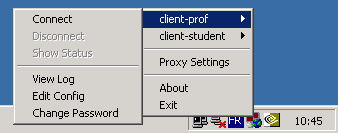
\includegraphics[width=0.47\textwidth]{partie_2/images/openvpn-client-connect.png}\\
	\end{center}
	\caption{Client OpenVPN sous windows}
	\label{openvpn_screen_windows}
\end{figure}


\subsubsection{Bilan et limites de la solution}

Une fois passée la phase un peu fastidieuse de mise en place et de configuration du serveur, OpenVPN se révèle facile à installer et à utiliser. Côté serveur, une fois les phases de compilation, installation, configuration, génération des certificats et lien avec la base NIS accomplies, le travail d'administration est quasi nul et n'impose plus que de regénérer les certificats de temps en temps.

Côté client la tâche est aisée, tout du moins sous Linux et Windows. Pour les autres systèmes la tâche peut se révéler complexe, mais le client a au moins le mérite d'exister et de fonctionner parfaitement.

La solution en elle même fournit un très bon niveau de sécurité. Les différents certificats permettent non seulement d'identifier les clients auprès du serveur, mais assurent également les clients qu'ils s'adressent bien au bon serveur. Pour finir l'authentification des clients est réalisée en faisant directement appel à l'annuaire de l'ISIMA.

En conclusion, OpenVPN est une solution mature et flexible qui rempli parfaitement le cahier des charges, tant du point de vue de la sécurité et de la méthode d'authentification que par son caractère multiplate-formes.


% \begin{figure}[H]
% 	\begin{center}
% 		\begin{minipage}{0.90\textwidth}
% 			\begin{lstlisting}[frame=trBL]
% 
% 			\end{lstlisting}
% 		\end{minipage}
% 	\end{center}
% 	\caption{Récupération des éléments de réponse dans un message de commande}
% 	\label{format_reponse_commande}
% \end{figure}
